\documentclass[12pt, oneside]{article}

\usepackage[utf8]{inputenc}
\usepackage[T1]{fontenc}
\usepackage{textcomp}
\usepackage{amsmath, amssymb}
\usepackage{fullpage}
\usepackage{graphicx}
\usepackage{amssymb, amsmath, amsthm}
\newtheorem{theorem}{Theorem}[section]
\newtheorem{corollary}{Corollary}[theorem]
\newtheorem{lemma}{Lemma}[theorem]
\title{Modeling Computer Viruses in Peer-to-Peer Networks}
\author{Abraham Porschet}
\date{\today}


% figure support
\usepackage{import}
\usepackage{xifthen}
\pdfminorversion=7
\usepackage{pdfpages}
\usepackage{transparent}

\pdfsuppresswarningpagegroup=1

\begin{document}
    \maketitle

    \section{Introduction}
        Peer to peer networks, caught on in the late 1990s and early 2000s with platforms like Limewire, Napster and MySpace. These websites
        were illustrative of the fun people could have with the internet, and also the malicious actions people could take using the internet.
        Peer to peer networks can be susceptible to various types of viruses, including self-propogating viruses such as the Samy worm \cite{VICE_2015}.\newline
        
        Obviously, the websites listed above have differences, but the main connection between them is that there are multiple users across a network
        who each have their own files or links or images publicly available for others to view or download. If a user wants to visit another user's 
        page or download another user's file(s), the user's web-client will have to connect with the other user and will then do what it was asked to do.\newline

        Some P2P networks, like Napster, have made it nearly impossibly to transmit infected files, but among other systems of the same class viruses have had a lot of success against networks like these, people can download things without being aware of it, and then viruses can download a payload to their 
        computer that adds itself to her files (so other people can download it by accident) and alters her system somehow. These viruses can behave quite similarly to 
        *actual* viruses. This means that a whole set of models, epidemiological models, are on the table to be used.\newline
        
        P2P (peer-to-peer) networks, used commercially, have millions of users that are connected in a web of millions of computer systems.
        In this web, file transfers happen rapidly, often in times much less than a second. When these webs encounter worms like the Samy worm
        or other similar viruses, they can propagate to thousands of users in very little time. If people are able to predict the spread of
        a virus inside of P2P networks, they are able to better respond to the virus at hand and better understand how to secure their network more.
        This modeling will take place in a simulation of P2P networks to assess a network's potential for propagation of viruses.\newline

        In Thommes and Coates paper on the same subject, they made the model assumption that the distribution of the infected files in the system was uniform. Essentially
        stating that each user has an equal likelihood of having an infected file, and that all users have the same expected number of infected files. However, all people are not equally
        likely to interact with infected files, or fall for internet-scams or viruses in general. In particular, the elderly have been shown to have a significantly higher risk factor for cyber
        threats, and the updated version of Thommes and Coates epidemiological model is presented here with a reflective update.

    \section{Methods and Model}
    
        The intent of the model is to approximate the spread of a computer virus that exists in a Peer-to-Peer (P2P) network. Note that we use the term user
        to refer to a person using a P2P client program. The term peer is used to collectively refer to a P2P client and the user directing its behaviour.
        The model examined \cite{1689197}, from Thommes and Coates, has peers of three types, Susceptible (S), Exposed (E), and Infected (I). 
    \subsection{Model}
        Since there are three different categories that a peer can fall into and each category is mutually exclusive with the others,
        it follows that at any time $t$, that  $N=S(t)+E(t)+I(t)$ where  $N$ is the number of peers in the system. We also make the assumption that the number of uninfected files is fixed at some $M$.
        The number of infected files at time  $t$ is given by a function  $K(t)$. When we then want to calculate the proportion of infected
        files to uninfected files, we get the proportion  $q(t)=\frac{K(t)}{M+K(t)}$. Thommes and Coates then assume that when a user interacts with a file,
        that it has a probability dependent on the number of infected files on the network and that the probability of an arbitrary file being infected is 
        time invariant, and is only dependent on the proportion $q(t)$, while I modeled the probability of a file being infected with a poisson distribution with
        probability mass function given by $P(K=k | \lambda) = \frac{e^{-\lambda}\lambda^k}{k!}$ where $K$ is a random variable representing the number of infected files
        infected by a peer and $k\in\mathbb{N}$ representing the number of files encountered and $\lambda(t)$ is a rate of of infected file encounters per minute. In this model we will
        have two different sub-populations. One population, representing people of lower risk of downloading files of dubious origin, or clicking on malicious links, will have a higher rate parameter,
        $\lambda_1$ and the other population, representing the lower risk population will have a lower rate parameter for interacting with malicious files, $\lambda_2$.
        We call the function that determines this probability  $f{q(t)}$. Then, for the last introduction of new variables, we have three
        other parameters for the following three actions: a peer downloading a file from another peer, a peer executing a shared file, 
        and a peer recovering. The parameters are then,  $\lambda_S$:  the rate in files per minute at which a peer downloads new files, 
        $\lambda_E$: average rate, in files per minute, at which each peer executes files, our last rate parameter is  $\lambda_R$:
        which is the average rate of recoveries per minute, at which infected peers recover. A recovery occurs when all infected files are
        removed, returning the peer to susceptible. The state cycle of this model is  $S\to E\to I \to S\ldots$\newline

        According to the 2022 Census, just over 17\% of Americans are over 65\cite{uscensus2022}. These people are at a significantly higher risk for 
        cyber crimes and general security breaches\cite{blackwood-brown2018}. Similarly, people under the age of 15 are also at significant risk. 
        Some estimates of their risk factor, have the elderly at up to 10 times higher
        risk for clicking on malicous links and other similar attacks, all of which are present on P2P systems which are examined here. For this reason, we will set
        $\lambda_1 = 10\lambda_2$, and then we can adjust $\lambda_2$ and see how it affects the behavior of the system. While fewer studies have derived estimates for
        younger populations, we assume it is something similar. 

        We now derive our differential equations.
        \subsubsection{Rate at Which Infected Peers Change}
        When infected peers change back to susceptible,  $I$ decreases by 1. Recoveries occur at rate  $\lambda_R I(t)$.
        Similarly, when an exposed person executes a file, they become infected and this happens at the rate $\lambda_E E(t)$, which
        gives us our first differential equation \[
        \frac{dI(t)}{dt}=-\lambda_R I(t)+\lambda_E E(t)
        \] 
        \subsubsection{Rate at Which Exposed Peers Change}
        The rate that exposed peers decrease due to infection, is just the negative of the $E(t)$ term from the last differential equation.
        The rate at which susceptible peers are exposed is dependent on the rate at which they download files, multiplied by the probability
        that a given file is infected. This gives us a rate of \[
            \frac{dE(t)}{dt}=-\lambda_E E(t)+\lambda_S S(t)f{q(t)}
        \]
        \subsubsection{Rate at Which Susceptible Peers Change}
        This is determined by the negative of the first term of the first equation and the negative of the second term of the second equation, giving us
        \[
            \frac{dS(t)}{dt}=-\lambda_S S(t)f{q(t)}+\lambda_R I(t)
        \]
    \section{Results}
        Thommes and Coates did their simulations as written above with a uniform distribution while the main difference between our simulations was the probability distribution chosen.
        Since some accounts might only have infected files, existing with the goal to only infect other accounts and plenty of clean accounts, I figured that a poisson distribution
        would be a better choice for modeling the infected files per peer. Now, if we use the expectation of that distribution in order to model the spread of some 
        virus over a peer to peer network, we the formula for the probability mass function for the poisson, with the parameter (generally seen as $\lambda$) $q(t)$ as described in the 
        methods section. In order to see how the difference in distribution affects the behavior of the system, we take the same initial conditions as described in Thommes and Coates paper
        and simulate the virus in a network.\newline

        With the initial conditions describes in Thommes and Coates, with $\lambda_E = \lambda_S=3.47\times 10^{-3}$ files per minute (5 downloads per day). Then we consider the average recovery
        time to be 24 hours, making $\lambda_R=6.94\times 10^{-4}$. The number of peers is 2 million and there are 60 million clean files, $M$. Initially there are 10,000 exposed files, all sharing one
        infected file. In the first figure we have $\lambda_1=5\times 10^{-4}$ and $\lambda_2=5\times 10^{-5}$ for the higher and lower rates respectively.
        \begin{figure}[htbp]
            \centering
            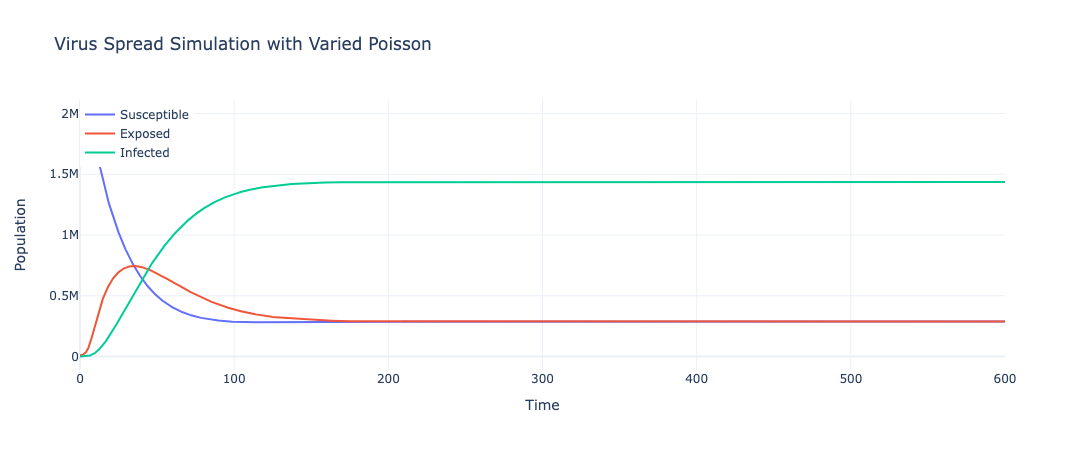
\includegraphics[width=0.9\textwidth]{2MPoisson.png}
            \caption{Image depicting initial conditions given by Thommes and Coates with varied Poisson distribution.}
        \end{figure}

        \begin{figure}[htbp]
            \centering
            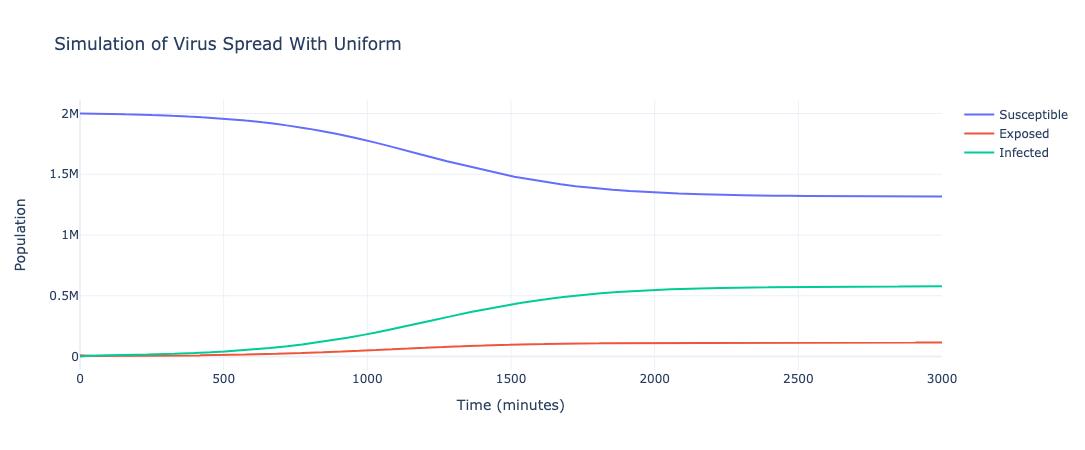
\includegraphics[width=0.9\textwidth]{2MUniform.png}
            \caption{Image depicting initial conditions given by Thommes and Coates with Uniform distribution.}
        \end{figure}
        These models actually appear diverge significantly. The model equipped with the varied poisson distribution seems to show that generic viruses present more of a threat than expected by Thommes and Coates
        with their paper. Even when you decrease the number of exposed peers, or the number of infected files in the system, the system hits a steady state result where
        most of the users are infected and there are a minority of peers that are not infected or exposed at any point. However, if you half the time it takes to recover, the system looks much more similar to the
        system given with the uniform distribution and the otherwise identical conditions. This indicates that by one metric, these viruses are at least 2 times more dangerous than expected. This is probably because
        if one group, even if they are a minority of the population is taking on malware more quickly than any other group of the population, they will have so many malicious files that almost any interaction with them
        will lead to a switch from susceptible to exposed or to infected. So while they might not be a majority of the population, we can clearly see that having a vulnerable minority puts the entire group at risk.

        Another interesting factor with using the alternate distribution is that the time to convergence doesn't seem to increase even if the number of initially exposed peers is decreased by multiple orders of magnitude \textit{and}
        the number of total files is increased by an order of magnitude. When you look at the graph, it looks essentially identical to the graph given by the initial conditions given by Thommes and Coates except that the axes are completely
        different.
        \begin{figure}[htbp]
            \centering
            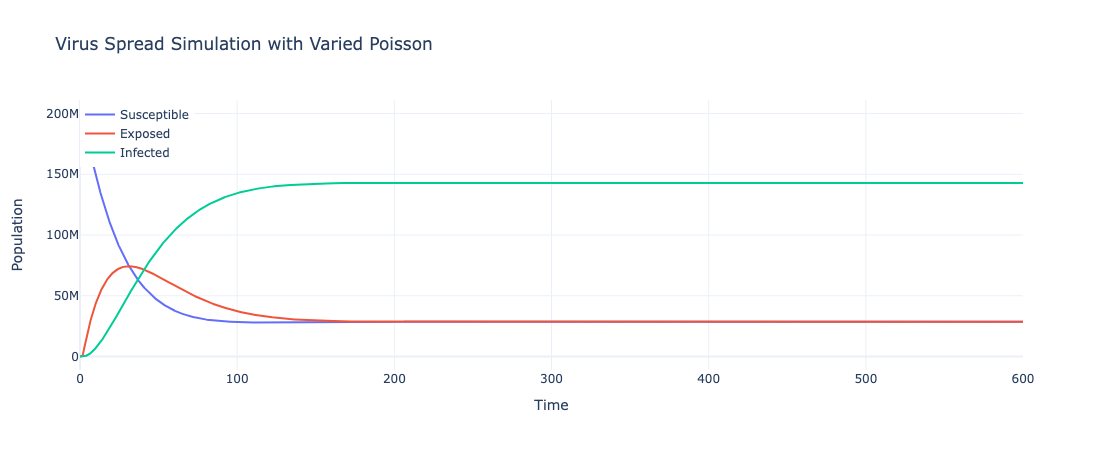
\includegraphics[width=0.9\textwidth]{HUGESUSCEPTIBLEPOISSON.png}
            \caption{varied poisson with the ratio of bad files $10^3$ times smaller and the number of exposed peers 100 times smaller }
        \end{figure}
    
    \section{Conclusion}
        The model described has shown that the propagation of computer viruses on P2P networks is possibly more dangerous than predicted by mathematicians such as Thommes and Coates if
        you account for the increased danger certain subsets of the population face. I also witnessed some really odd behaviors about the time it takes to hit the steady state for the system 
        equipped with the poisson distribution. Finding a closed form formula for the convergence of the system is much more difficult with another distribution equipped, 
        than it is with the uniform distribution, but that would be a useful next step for future work. Finding a closed form solution would also help understand the question about why the 
        steady state is reached at approximately the same time regardless of concentration of infected files. Along with that would be actual physical tests with a worm or 'malicious' file that is generally benign,
        and then track how it propagates across a network and use that research in order to craft models that are potentially more accurate and use them to verify the changes in rate parameters or statistical
        distributions used.
    \section{Acknowledgements}
        I'd like to thank Monica and Cara for giving me advice to look further into the assumptions I was making about the demographics of the systems I was looking at as well as helping with some spelling mistakes.

\bibliography{paper}
\bibliographystyle{plain}
\end{document}
